\documentclass{standalone}
\usepackage{tikz}
\usetikzlibrary{patterns, positioning}
\usepackage[sfdefault]{ClearSans} %% option 'sfdefault' activates Clear Sans as the default text font
\usepackage[T1]{fontenc}

\begin{document}
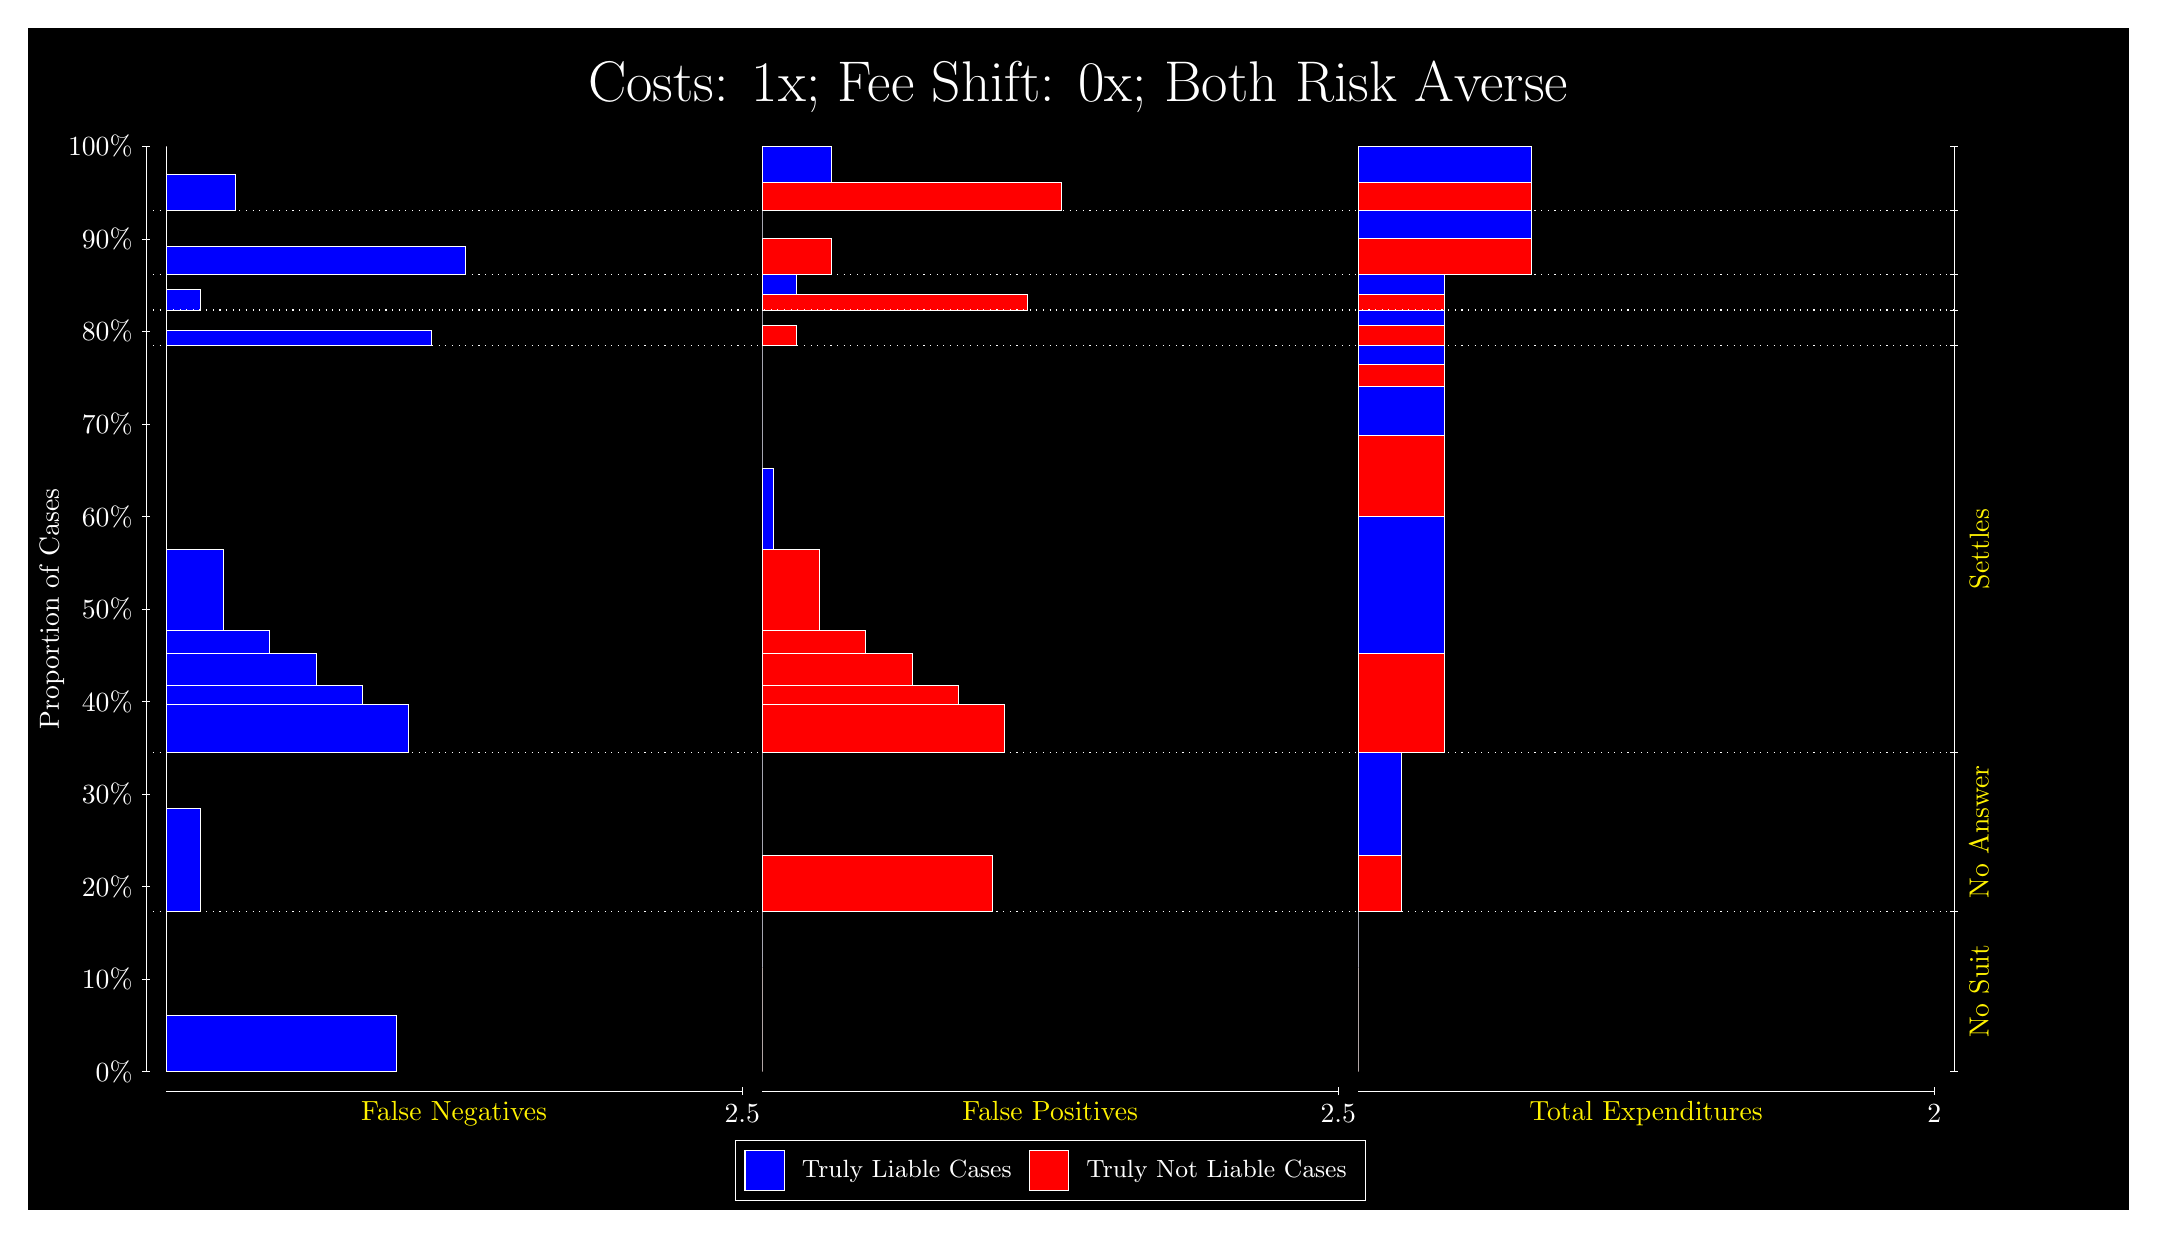
\begin{tikzpicture}
\draw[fill=black] (0,0) rectangle (26.667,15);
\draw[text=white] (0,13.5) rectangle (26.667,15) node[midway] {\huge Costs: 1x; Fee Shift: 0x; Both Risk Averse};
\draw[white, very thin] (1.5,1.75) -- (1.5,13.5);
\node[rotate=90, text=white, anchor=center] at (0.3, 7.625) {Proportion of Cases};
\draw[white, very thin] (1.45,1.75) -- (1.55,1.75);
\node[text=white, anchor=east] at (1.45, 1.75) {0\%};
\draw[white, very thin] (1.45,2.925) -- (1.55,2.925);
\node[text=white, anchor=east] at (1.45, 2.925) {10\%};
\draw[white, very thin] (1.45,4.1) -- (1.55,4.1);
\node[text=white, anchor=east] at (1.45, 4.1) {20\%};
\draw[white, very thin] (1.45,5.275) -- (1.55,5.275);
\node[text=white, anchor=east] at (1.45, 5.275) {30\%};
\draw[white, very thin] (1.45,6.45) -- (1.55,6.45);
\node[text=white, anchor=east] at (1.45, 6.45) {40\%};
\draw[white, very thin] (1.45,7.625) -- (1.55,7.625);
\node[text=white, anchor=east] at (1.45, 7.625) {50\%};
\draw[white, very thin] (1.45,8.8) -- (1.55,8.8);
\node[text=white, anchor=east] at (1.45, 8.8) {60\%};
\draw[white, very thin] (1.45,9.975) -- (1.55,9.975);
\node[text=white, anchor=east] at (1.45, 9.975) {70\%};
\draw[white, very thin] (1.45,11.15) -- (1.55,11.15);
\node[text=white, anchor=east] at (1.45, 11.15) {80\%};
\draw[white, very thin] (1.45,12.325) -- (1.55,12.325);
\node[text=white, anchor=east] at (1.45, 12.325) {90\%};
\draw[white, very thin] (1.45,13.5) -- (1.55,13.5);
\node[text=white, anchor=east] at (1.45, 13.5) {100\%};

\draw[white, very thin] (24.457,1.75) -- (24.457,13.5);
\draw[white, very thin] (24.407,1.75) -- (24.507,1.75);
\node[anchor=west] at (24.407, 1.75) {};
\draw[white, very thin] (24.407,3.7857) -- (24.507,3.7857);
\node[anchor=west] at (24.407, 3.7857) {};
\draw[white, very thin] (24.407,5.8033) -- (24.507,5.8033);
\node[anchor=west] at (24.407, 5.8033) {};
\draw[white, very thin] (24.407,10.967) -- (24.507,10.967);
\node[anchor=west] at (24.407, 10.967) {};
\draw[white, very thin] (24.407,11.422) -- (24.507,11.422);
\node[anchor=west] at (24.407, 11.422) {};
\draw[white, very thin] (24.407,11.876) -- (24.507,11.876);
\node[anchor=west] at (24.407, 11.876) {};
\draw[white, very thin] (24.407,12.688) -- (24.507,12.688);
\node[anchor=west] at (24.407, 12.688) {};
\draw[white, very thin] (24.407,13.5) -- (24.507,13.5);
\node[anchor=west] at (24.407, 13.5) {};

\draw[white, very thin, fill=blue] (1.75,1.75) rectangle (4.6775,2.4674);
\draw[white, very thin, fill=red] (1.75,2.4674) rectangle (1.75,3.7857);
\draw[white, very thin, fill=blue] (1.75,3.7857) rectangle (2.1891,5.0949);
\draw[white, very thin, fill=red] (1.75,5.0949) rectangle (1.75,5.8033);
\draw[white, very thin, fill=blue] (1.75,5.8033) rectangle (4.8239,6.4187);
\draw[white, very thin, fill=blue] (1.75,6.4187) rectangle (4.2384,6.6492);
\draw[white, very thin, fill=blue] (1.75,6.6492) rectangle (3.6529,7.0675);
\draw[white, very thin, fill=blue] (1.75,7.0675) rectangle (3.0674,7.3578);
\draw[white, very thin, fill=blue] (1.75,7.3578) rectangle (2.4819,8.3854);
\draw[white, very thin, fill=red] (1.75,8.3854) rectangle (1.75,10.967);
\draw[white, very thin, fill=blue] (1.75,10.967) rectangle (5.1167,11.163);
\draw[white, very thin, fill=red] (1.75,11.163) rectangle (1.75,11.422);
\draw[white, very thin, fill=blue] (1.75,11.422) rectangle (2.1891,11.68);
\draw[white, very thin, fill=red] (1.75,11.68) rectangle (1.75,11.876);
\draw[white, very thin, fill=blue] (1.75,11.876) rectangle (5.5558,12.234);
\draw[white, very thin, fill=red] (1.75,12.234) rectangle (1.75,12.688);
\draw[white, very thin, fill=blue] (1.75,12.688) rectangle (2.6283,13.141);
\draw[white, very thin, fill=red] (1.75,13.141) rectangle (1.75,13.5);
\draw[white, very thin, fill=red] (9.3189,1.75) rectangle (9.3189,3.0683);
\draw[white, very thin, fill=blue] (9.3189,3.0683) rectangle (9.3189,3.7857);
\draw[white, very thin, fill=red] (9.3189,3.7857) rectangle (12.246,4.4941);
\draw[white, very thin, fill=blue] (9.3189,4.4941) rectangle (9.3189,5.8033);
\draw[white, very thin, fill=red] (9.3189,5.8033) rectangle (12.393,6.4187);
\draw[white, very thin, fill=red] (9.3189,6.4187) rectangle (11.807,6.6491);
\draw[white, very thin, fill=red] (9.3189,6.6491) rectangle (11.222,7.0675);
\draw[white, very thin, fill=red] (9.3189,7.0675) rectangle (10.636,7.3579);
\draw[white, very thin, fill=red] (9.3189,7.3579) rectangle (10.051,8.3854);
\draw[white, very thin, fill=blue] (9.3189,8.3854) rectangle (9.4652,9.4129);
\draw[white, very thin, fill=blue] (9.3189,9.4129) rectangle (9.3189,10.967);
\draw[white, very thin, fill=red] (9.3189,10.967) rectangle (9.758,11.226);
\draw[white, very thin, fill=blue] (9.3189,11.226) rectangle (9.3189,11.422);
\draw[white, very thin, fill=red] (9.3189,11.422) rectangle (12.686,11.617);
\draw[white, very thin, fill=blue] (9.3189,11.617) rectangle (9.758,11.876);
\draw[white, very thin, fill=red] (9.3189,11.876) rectangle (10.197,12.329);
\draw[white, very thin, fill=blue] (9.3189,12.329) rectangle (9.3189,12.688);
\draw[white, very thin, fill=red] (9.3189,12.688) rectangle (13.125,13.046);
\draw[white, very thin, fill=blue] (9.3189,13.046) rectangle (10.197,13.5);
\draw[white, very thin, fill=red] (16.888,1.75) rectangle (16.888,3.0683);
\draw[white, very thin, fill=blue] (16.888,3.0683) rectangle (16.888,3.7857);
\draw[white, very thin, fill=red] (16.888,3.7857) rectangle (17.437,4.4941);
\draw[white, very thin, fill=blue] (16.888,4.4941) rectangle (17.437,5.8033);
\draw[white, very thin, fill=red] (16.888,5.8033) rectangle (17.986,7.0675);
\draw[white, very thin, fill=blue] (16.888,7.0675) rectangle (17.986,8.8037);
\draw[white, very thin, fill=red] (16.888,8.8037) rectangle (17.986,9.8313);
\draw[white, very thin, fill=blue] (16.888,9.8313) rectangle (17.986,10.447);
\draw[white, very thin, fill=red] (16.888,10.447) rectangle (17.986,10.737);
\draw[white, very thin, fill=blue] (16.888,10.737) rectangle (17.986,10.967);
\draw[white, very thin, fill=red] (16.888,10.967) rectangle (17.986,11.226);
\draw[white, very thin, fill=blue] (16.888,11.226) rectangle (17.986,11.422);
\draw[white, very thin, fill=red] (16.888,11.422) rectangle (17.986,11.617);
\draw[white, very thin, fill=blue] (16.888,11.617) rectangle (17.986,11.876);
\draw[white, very thin, fill=red] (16.888,11.876) rectangle (19.083,12.329);
\draw[white, very thin, fill=blue] (16.888,12.329) rectangle (19.083,12.688);
\draw[white, very thin, fill=red] (16.888,12.688) rectangle (19.083,13.046);
\draw[white, very thin, fill=blue] (16.888,13.046) rectangle (19.083,13.5);
\draw[white, dotted] (1.5,3.7857) -- (24.457,3.7857);
\draw[white, dotted] (1.5,5.8033) -- (24.457,5.8033);
\draw[white, dotted] (1.5,10.967) -- (24.457,10.967);
\draw[white, dotted] (1.5,11.422) -- (24.457,11.422);
\draw[white, dotted] (1.5,11.876) -- (24.457,11.876);
\draw[white, dotted] (1.5,12.688) -- (24.457,12.688);
\draw[white, very thin] (1.75,1.5) -- (9.0689,1.5);
\node[text=yellow, anchor=north] at (5.4094, 1.5) {False Negatives};
\draw[white, very thin] (9.0689,1.45) -- (9.0689,1.55);
\node[text=white, anchor=north] at (9.0689, 1.45) {2.5};

\draw[white, very thin] (9.3189,1.5) -- (16.638,1.5);
\node[text=yellow, anchor=north] at (12.978, 1.5) {False Positives};
\draw[white, very thin] (16.638,1.45) -- (16.638,1.55);
\node[text=white, anchor=north] at (16.638, 1.45) {2.5};

\draw[white, very thin] (16.888,1.5) -- (24.207,1.5);
\node[text=yellow, anchor=north] at (20.547, 1.5) {Total Expenditures};
\draw[white, very thin] (24.207,1.45) -- (24.207,1.55);
\node[text=white, anchor=north] at (24.207, 1.45) {2};

\node[text=yellow, centered, rotate=90] at (24.777, 2.7678) {No Suit};
\node[text=yellow, centered, rotate=90] at (24.777, 4.7945) {No Answer};
\node[text=yellow, centered, rotate=90] at (24.777, 8.3854) {Settles};





\draw (12.978300999999998,1.5) node[draw=none] (baseCoordinate) {};
\begin{scope}[align=center]
        \matrix[scale=0.5, draw=white, below=0.5cm of baseCoordinate, nodes={draw}, column sep=0.1cm]{
            \node[rectangle, draw, minimum width=0.5cm, minimum height=0.5cm, fill=blue] {}; &
            \node[draw=none, font=\small, text=white] (B) {Truly Liable Cases}; &
            \node[rectangle, draw, minimum width=0.5cm, minimum height=0.5cm, fill=red] {}; &
            \node[draw=none, font=\small, text=white] (B) {Truly Not Liable Cases}; \\
            };
\end{scope}

\end{tikzpicture}
\end{document}